\chapter{Proposta de Dissertação}
\label{sec:prop_sis_rec_exp}

Este capítulo apresenta a motivação, os objetivos, a metodologia, trabalhos preliminares, o empacotamento, a avaliação, as contribuições esperadas e o cronograma para o desenvolvimento desta proposta de dissertação de mestrado.

\section{Motivação}
\label{sec:moti}
Realizar um experimento em LPS exige alguns pontos de atenção específicos para garantir a qualidade do experimento. Estes pontos tem sido investigados em um trabalho de mestrado em andamento do nosso Grupo de pesquisa em Reuso Sistemático de Software e Experimentação (GRSSE), neste trabalho vem sendo elaborado diretrizes para a determinar a qualidade de experimentos em LPS. Esta tarefa possui um árduo trabalho para garantir que, aspectos específicos do domínio como, por exemplo, os artefatos utilizados que são, os objetos experimentais, a complexidade do treinamento, a dificuldade de seleção de participantes qualificados em LPS e a falta de repositórios de LPS, não influenciem nos experimentos ao ponto de invalidá-los. A falta de experimentos com qualidade afeta diretamente a possibilidade de repetição dos estudos em LPS.

Sabendo que para realizar um experimento em LPS com qualidade exige-se seguir alguns modelos e diretrizes, construir um sistema de recomendação que recomende métodos, processos, diretrizes, entre outros, para realizar um experimento em LPS, pode proporcionar facilidade ao desenvolvimento dos mesmos, incentivando a cultura e desenvolvimento de experimentos na academia e industria.

Por meio do GRSSE, foi encontrada uma lacuna nas pesquisas de qualidade em experimentos de ES em LPS que proporciona esta pesquisa, apresentando um campo aberto à pesquisa para determinar qualidade e recomendação para experimentos em LPS.


\section{Objetivos}
\label{sec:obj}

Esta pesquisa tem como objetivo geral especificar e implementar um sistema de recomendação para experimentos em LPS caracterizados por sua qualidade

Os objetivos específicos deste projeto são:

\begin{itemize}
	\item gerar e representar um conjunto de meta dados a partir das informações sobre experimentos em LPS;
	\item definir técnicas de recomendação com base nos meta dados;
	\item projeto e desenvolvimento do sistema de recomendação e;
	\item avaliar e empacotar o sistema de recomendação.
\end{itemize}

\section{Metodologia}
\label{sec:meto}

O processo de execução deste trabalho para chegar ao objetivo será, pesquisar de maneira exploratória um modelo de sistema de recomendação em experimentos de LPS. Para tal resultado será desenvolvido um projeto de software e em seguida executado o mesmo. A \ref{fig:metodologia_flow} apresenta as etapas de desenvolvimento desta pesquisa.

\begin{figure}[htb]
	\centering					
	{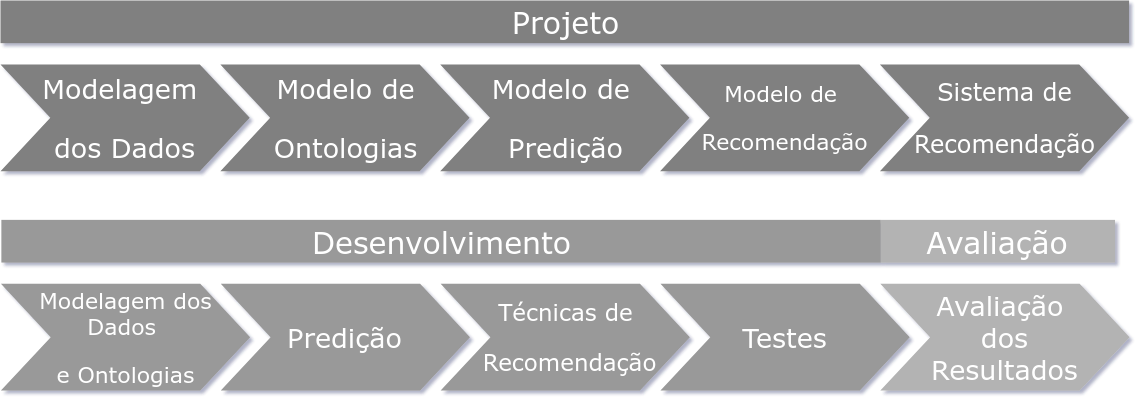
\includegraphics[scale=.4]{metodologia_flow.png}}
	
	\caption{Etapas da Metodologia de Desenvolvimento de Pesquisa}
	\label{fig:metodologia_flow}
\end{figure}

Neste projeto de pesquisa vamos levantar uma base de dados sobre a qualidade de experimentos em LPS. Por meio desta base será possível gerar um modelo de dados baseado em ontologias, \textbf{TBox} e \textbf{ABox}, com o objetivo de extrair informações preditivas desta base. Após processar essas informações baseada nos meta dados de qualidade de experimentos em LPS, será possível criar um sistema de recomendação, utilizando as ferramentas apropriadas de recomendação em ES.

\begin{itemize}
	\item \textbf{O Papel da Ontologia:} será de estruturar e modelar a base de informações extraída do Mapeamento Sistemático de experimentos em LPS que está sendo desenvolvido pelo GRSSE. Pode se dizer que este modelo será o conjunto de meta dados;
	
	\item \textbf{O Papel do Sistema de Recomendação:} será de interagir com o usuário afim de extrair informações relevantes, de modo que se possa determinando o deste perfil do usuário, para que possa ser realizada inferências no modelo ontológico de diretrizes de qualidade gerando recomendações de métodos, processos, diretrizes para o experimento do usuário.
\end{itemize}

O desenvolvimento do projeto, inclui realizar a escolha das tecnologias a serem usadas como ferramenta de construção do software, como por exemplo, as linguagens de programação, o ambiente de desenvolvimento, a diagramação do projeto, os \textit{stakeholders} envolvidos no projeto, ferramentas de \textit{Application Lifecycle Management} (ALM) aplicadas ao escopo do projeto, escolha das abordagens de sistemas de recomendação, definição do modelo de ontologias, definição da base de dados para representação tanto, dos dados de origem (itens, usuários), quanto, para representação dos dados para apresentação e armazenamento dos resultados obtidos da recomendação. 

Após a definição do projeto de software, inicia-se o processo de desenvolvimento do sistema de recomendação. Com o auxílio de ferramentas de ALM será possível acompanhar por todos os \textit{stakeholders} envolvidos o desenvolvimento online da ferramenta, desta forma se tornando um processo mais colaborativo entre eles. Inicialmente será realizado a modelagem dos dados extraído da avaliação de qualidade dos experimentos em LPS realizado pelo trabalho do GRSSE, que são 174 experimentos encontrado na literatura nesse ramo de pesquisa. Em seguida será aplicado um modelo de ontologia definido no projeto de software, nesta base de informações de experimentos, tem como propósito, realizar predições para um modelo mais abstrato sobre qualidade de experimentos em LPS. Na sequência será desenvolvido o modelo de recomendação, este desenvolvimento consiste na modelagem dos dados encontrado na predição da ontologia para extrair as informações necessárias para o modelo de recomendação, posteriormente aplicar os algoritmos neste modelo. Em seguida será desenvolvido um \textit{front-end} de interação com o usuário poder dar entrada na informações iniciais para gerar as recomendações. O último passo será realizado um estudo para avaliação deste sistema de recomendação.

\begin{figure}[htb]
	\centering					
	{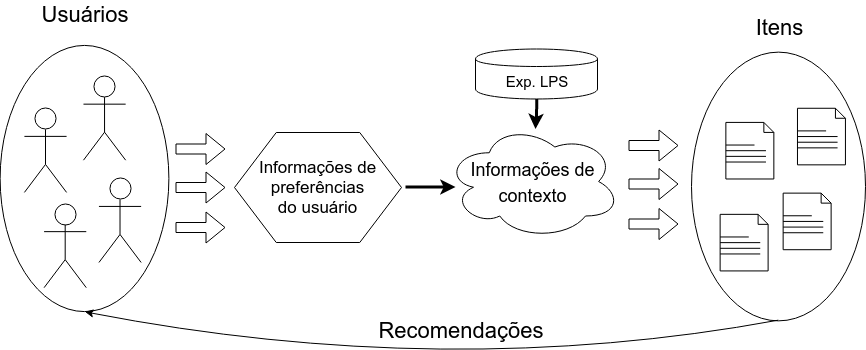
\includegraphics[scale=.5]{RSSE-overview.png}}
	
	\caption{Modelagem geral da RSSE proposta}
	\label{fig:RSSE-overview}
\end{figure}

A \ref{fig:RSSE-overview} apresenta o conceito geral da metodologia deste projeto. Iniciando pela entrada dos usuários, depois extraímos as preferencias dele, e em seguida será feita a extração de informações de contexto utilizando a base de meta dados em LPS, para então fazer inferência nos itens (que são experimentos em LPS), por meio dessa inferência será obtido as recomendações.

Inicialmente, a entrada de dados dos usuários está sendo definido da seguinte forma:

\begin{itemize}
	\item Informações de LPS:
		\subitem Dominio;
		\subitem Sub-dominio;
		\subitem Tipos de artefatos e;
		\subitem Feature module.
	\item Experimentos
		\subitem filtrar por qualidade.
\end{itemize}


\section{Trabalhos Preliminares}

\subsection{Transformação de planilha para banco de dados}

A extração de dados a partir da planilha de Excel da revisão sistemática do GRSSE. Para esta transformação está sendo utilizando uma ferramenta de ETL (\textit{Extract, Transform, Load}) chamada PDI (\textit{Pentaho Data Integration}) transportando os dados da planilha para um banco de dados relacional (MySql).

A \ref{fig:etl-meta-dados} do Apêndice \ref{apen:a1}, apresenta o esta transformação em construção, este processo é realizado por meio de uma leitura linha-a-linha da planilha e persistindo em uma tabela na base de dados MySql previamente definida.

\subsection{Grafo inicial de diretrizes para base ontológica de qualidade de experimentos em LPS}

Para levantar as diretrizes iniciais da ontologia (\textbf{TBox} e \textbf{ABox}), está sendo desenvolvido um grafo usando uma ferramenta de mapa mental (Xmind), mapeando as possíveis classificações e suas tipagens bem como alguns exemplos de informações inerentes aos domínios classificados.

Esta construção inicial pode ser visto na \ref{fig:diretrizes-01} do Apêndice \ref{apen:a3}, e com exemplos iniciais na \ref{fig:diretrizes-03} do Apêndice \ref{apen:a3}. Para concluir esta etapa falta filtrar as classes que realmente representam uma relevância para qualidade em LPS e cria os relacionamento entre estas classes de domínios.

\subsection{SQL para listar diretrizes comuns}
Para auxiliar na extração de informações das classificação de domínio da ontologia, foi desenvolvidos sete \textit{querys} (como pode ser visto no Apêndice \ref{apen:a2}) para formar uma base inicial de dados (\textbf{ABox}) do nosso modelo ontológico.


\section{Empacotamento}

Todo projeto está sendo versionado no Github pelo link: https://github.com/rickvig/pcc-pesquisa.


\section{Avaliação}
\label{sec:aval}
Na Literatura é possível encontrar algumas dimensões para avaliação de RSSE, e as recomendações providas por ele. Em \citet{robillard2010recommendation} são apresentadas 16 dimensões de avaliação para um RSSE, que estão apresentadas na \ref{tab:dimensoes}. Cada dimensão possui sua técnica de avaliação, algumas são quantitativas outras qualitativas, algumas possuem as duas abordagens.

\begin{table}[]
	\centering
	\caption{Dimensões de avaliação para RSSE. Tradução de \citet{robillard2010recommendation}}
	\label{tab:dimensoes}
	\begin{tabular}{|l|l|l|ll}
		\cline{1-3}
		\multicolumn{1}{|c|}{\cellcolor[HTML]{C0C0C0}\textbf{Dimensão}} & \multicolumn{1}{c|}{\cellcolor[HTML]{C0C0C0}\textbf{Descrição}} & \multicolumn{1}{c|}{\cellcolor[HTML]{C0C0C0}\textbf{Tipo de métrica}} &  &  \\ \cline{1-3}
		Corretude & \begin{tabular}[c]{@{}l@{}}Quão próximo é a recomendação do \\ conjunto de recomendações que \\ assumimos ser corretas?\end{tabular} & quantitativa &  &  \\ \cline{1-3}
		Cobertura & \begin{tabular}[c]{@{}l@{}}Até que ponto a cobertura do SR sobre \\ um conjunto de itens ou o espaço do usuário?\end{tabular} & quantitativa &  &  \\ \cline{1-3}
		Diversidade & Qual a diversidade das recomendações? & quantitativa &  &  \\ \cline{1-3}
		Confiável & Como a recomendação pode ser confiável? & qualitativa &  &  \\ \cline{1-3}
		Confiança do SR & Quão confiante o SR é? & \begin{tabular}[c]{@{}l@{}}quantitativa / \\ qualitativa\end{tabular} &  &  \\ \cline{1-3}
		Novidade & \begin{tabular}[c]{@{}l@{}}Qual é o sucesso do SR em gerar novas \\ recomendações ou recomendações ainda \\ desconhecidas para o usuário?\end{tabular} & \begin{tabular}[c]{@{}l@{}}quantitativa / \\ qualitativa\end{tabular} &  &  \\ \cline{1-3}
		Acaso & \begin{tabular}[c]{@{}l@{}}Até que ponto o SR ainda promove \\ surpresa com sucesso?\end{tabular} & \begin{tabular}[c]{@{}l@{}}quantitativa /\\ qualitativa\end{tabular} &  &  \\ \cline{1-3}
		Utilidade & \begin{tabular}[c]{@{}l@{}}Qual é o ganho de valor dessa \\ recomendação para o usuário?\end{tabular} & \begin{tabular}[c]{@{}l@{}}quantitativa / \\ qualitativa\end{tabular} &  &  \\ \cline{1-3}
		Risco & \begin{tabular}[c]{@{}l@{}}Qual é o risco para o usuário \\ aceitar essa recomendação?\end{tabular} & qualitativa &  &  \\ \cline{1-3}
		Robustez & \begin{tabular}[c]{@{}l@{}}Qual é a tolerância do SR para um \\ viés ou uma informação falsa?\end{tabular} & quantitativa &  &  \\ \cline{1-3}
		\begin{tabular}[c]{@{}l@{}}Taxa de \\ Aprendizagem\end{tabular} & \begin{tabular}[c]{@{}l@{}}Quão rápido é o SR para adicionar novas \\ informações ou atualizar a lista de recomendação?\end{tabular} & quantitativa &  &  \\ \cline{1-3}
		Usabilidade & \begin{tabular}[c]{@{}l@{}}O qual usável é o SR? Será fácil dos \\ usuários se adequar de uma forma apropriada?\end{tabular} & \begin{tabular}[c]{@{}l@{}}quantitativa / \\ qualitativa\end{tabular} &  &  \\ \cline{1-3}
		Escalabilidade & \begin{tabular}[c]{@{}l@{}}Quão escalável é o SR em relação \\ ao numero de usuários, levando em \\ consideração o tamanho dos dados e \\ a performance dos algoritmos?\end{tabular} & quantitativa &  &  \\ \cline{1-3}
		Estabilidade & Quão consistente é o SR em um período de tempo? & quantitativa &  &  \\ \cline{1-3}
		Privacidade & Existe algum risco a privacidade do usuário? & \begin{tabular}[c]{@{}l@{}}quantitativa / \\ qualitativa\end{tabular} &  &  \\ \cline{1-3}
		\begin{tabular}[c]{@{}l@{}}Preferência do\\ Usuário\end{tabular} & Como o usuário entende o SR? & \begin{tabular}[c]{@{}l@{}}quantitativa / \\ qualitativa\end{tabular} &  &  \\ \cline{1-3}
	\end{tabular}
\end{table}

\begin{table}[]
	\centering
	\caption{Categorização das 16 dimensões. Tradução de \citet{robillard2010recommendation}}
	\label{tab:dimens-catg}
	\begin{tabular}{@{}llll@{}}
		\toprule
		\begin{tabular}[c]{@{}l@{}}Centralizado na \\ Recomendação\end{tabular} & \begin{tabular}[c]{@{}l@{}}Centralizado no \\ Usuário\end{tabular} & \begin{tabular}[c]{@{}l@{}}Centralizado no \\ Sistema\end{tabular} & \begin{tabular}[c]{@{}l@{}}Centralizado na \\ Entrega\end{tabular} \\ \midrule
		Corretude & Confiável & Robustez & Usabilidade \\
		Cobertura & Novidade & Taxa de Aprendizagem & Preferência do usuário \\
		Diversidade & Acaso & Escalabilidade &  \\
		Confiança do SR & Utilidade & Estabilidade &  \\
		& Risco & Privacidade &  \\ \bottomrule
	\end{tabular}
\end{table}

Essas dimensões podem ser subdivididas em categorias como mostra a \ref{tab:dimens-catg}. As dimensões centradas na recomendação avaliam principalmente as recomendações geradas pelo próprio sistema de recomendação. As dimensões centradas no usuário nos permitem avaliar se o sistema de recomendação atende às necessidades do seu usuário final. As dimensões centradas no sistema, em contraste a dimensões anterior, estas fornecem principalmente formas de avaliar o próprio sistema de recomendação ao invés das recomendações. Finalmente, as dimensões centradas na entrega estão focadas principalmente no contexto de uso do sistema de recomendação \cite{robillard2010recommendation}.

\begin{figure}[htb]
	\centering					
	{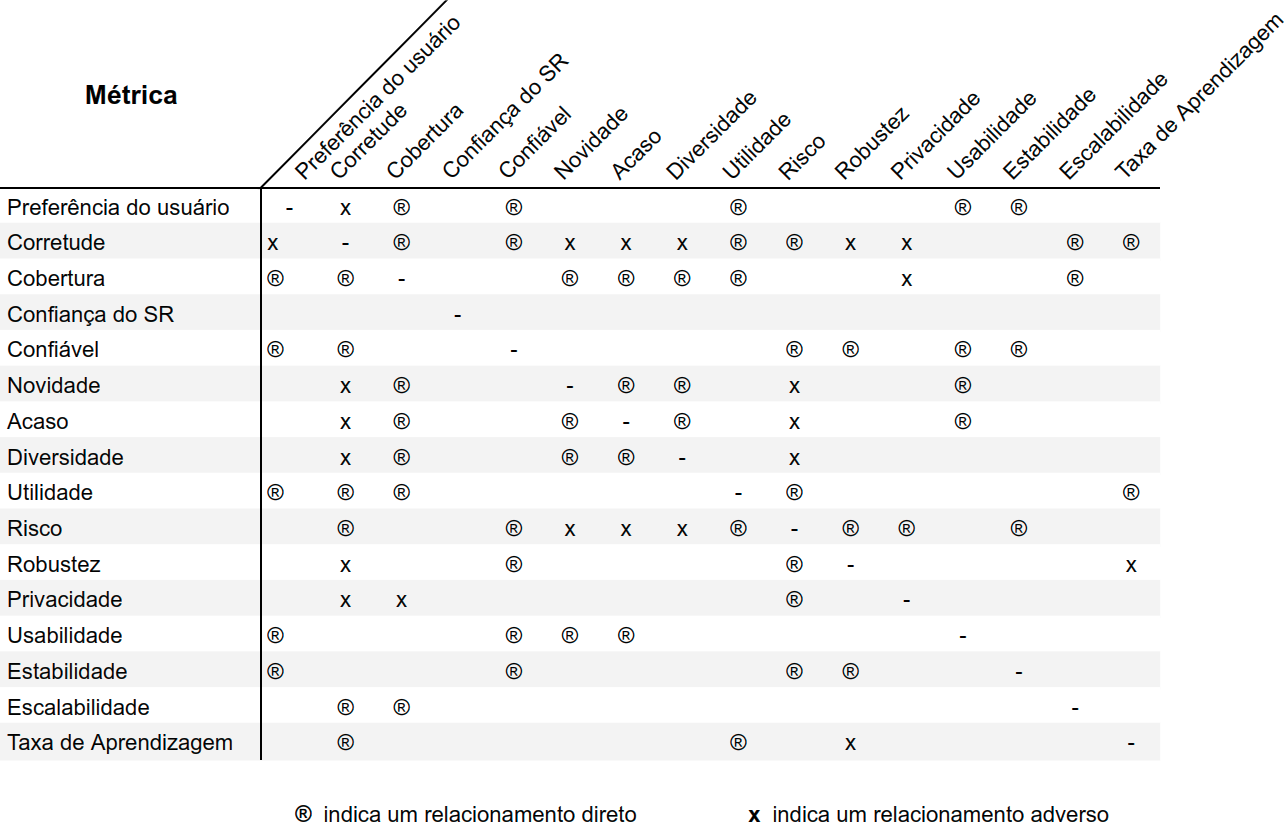
\includegraphics[scale=.4]{rel_metricas_pt.png}}
	
	\caption{Cruzamento de interesses entre as dimensões. Traduzido e adaptado de \citet{robillard2010recommendation}}
	\label{fig:rel_metricas}
\end{figure}

A \ref{fig:rel_metricas} apresenta o relacionamentos direto e adverso entro as métricas de avaliação. Por exemplo, o relacionamento direto entre as métricas Corretude e Cobertura, significa que, se o RSSE possui a métrica Corretude  provavelmente terá a métrica de Cobertura. No caso do relacionamento adverso, por exemplo, as métricas Corretude e Diversidade, significa que, se o RSSE possui a métrica Corretude provavelmente não terá a métrica Diversidade


\section{Contribuições Esperadas}
\label{sec:contr}

Espera-se que com este trabalho seja encontrado um modelo (projeto e implementação) de recomendação para experimentos de LPS. Espera-se também realizar um estudo de caso a fim de analisar o modelo proposto.

Espera-se que com esta pesquisa se inicie um processo de melhoramento na qualidade de experimentação em LPS, em que, possa ser realizado por meio deste projeto e implementação de sistema de recomendação.

Contribuir com a comunidade de LPS a projetar e executar experimentos melhores, desta forma aumentar a confiança do corpo de conhecimento visando a transferência de tecnologia para indústria.

\section{Cronograma}
\label{sec:cron}

As etapas que compõem o cronograma de execução desta proposta de projeto de dissertação de mestrado são descritas a seguir e apresentadas abaixo na \ref{fig:cronograma}, evidenciado as que estão em andamento a serem executadas e concluídas de acordo com legenda.

\begin{itemize}
	\item E1 - Revisão da Literatura
	\item E2 - Projeto: Tecnologias
	\item E3 - Projeto: Modelo de Ontologias
	\item E4 - Projeto: Modelo de Predição
	\item E5 - Projeto: Modelagem de dados
	\item E6 - Projeto: Modelo de Recomendação
	\item E7 - Projeto: Front-End
	\item E8 - Desenvolvimento: Ontologias
	\item E9 - Desenvolvimento: Predição
	\item E10 - Desenvolvimento: Recomendação
	\item E11 - Desenvolvimento: Front-End
	\item E12 - Testes
	\item E13 - Avaliação dos Resultados
	\item E14 - Escrever Qualificação
	\item E15 - Defesa da Qualificação
	\item E16 - Escrever Dissertação
	\item E17 - Defesa da Dissertação
	\item E18 - Escrita de artigos para conferencia e periódicos qualificados
\end{itemize}

\begin{figure}[]
	\centering					            
	{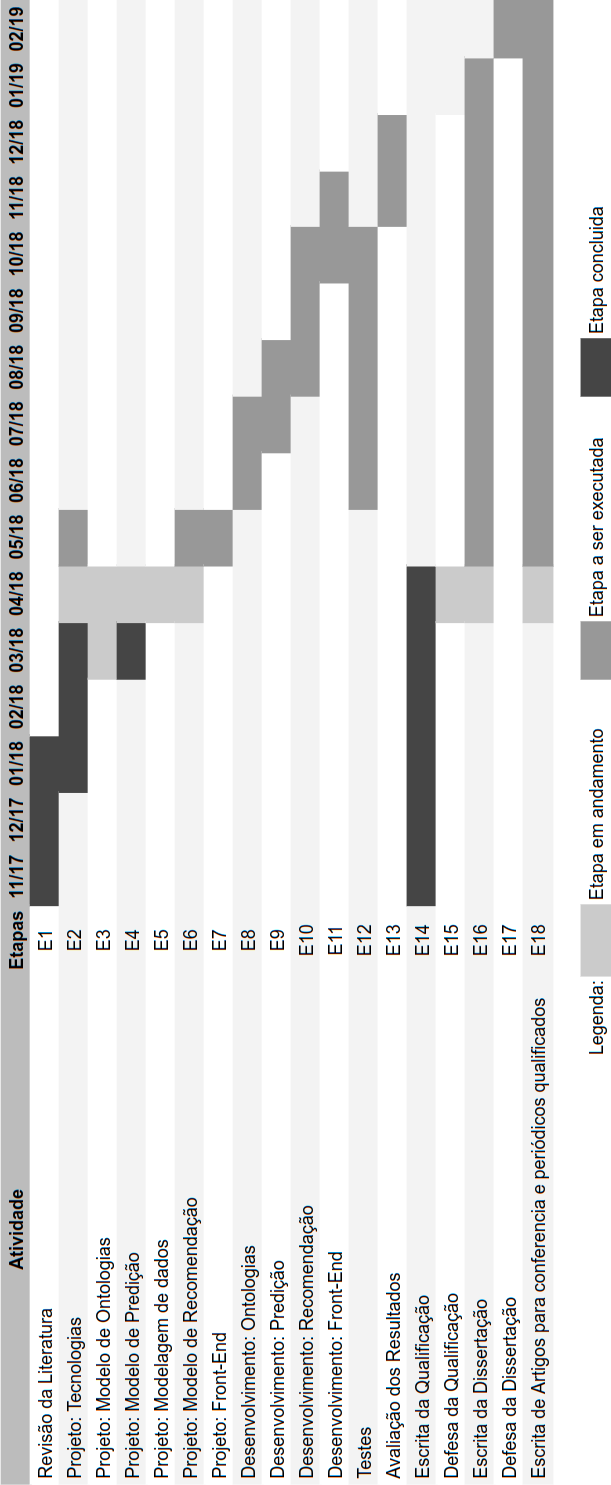
\includegraphics[scale=.45]{cronograma.png}}
	
	\caption{Cronograma de desenvolvimento da pesquisa - Anos 2018/2019}
	\label{fig:cronograma}
\end{figure}
